\documentclass[border=2pt]{standalone}
\usepackage{tikz}
\usetikzlibrary{arrows.meta,positioning,calc,fit,backgrounds,shapes.geometric}
\usepackage{amsmath,amssymb}
\usepackage{times}
\definecolor{ink}{HTML}{243447}
\definecolor{cA}{HTML}{4477AA}
\definecolor{cB}{HTML}{CC6677}
\definecolor{cAu}{HTML}{44AA99}
\definecolor{cS}{HTML}{CCAA33}
\definecolor{grn}{HTML}{228833}
\definecolor{rose}{HTML}{AA3377}
\definecolor{inst}{HTML}{F2E3B3}
\tikzset{
 pap/.style={circle,draw=ink,line width=.6pt,minimum size=15pt,inner sep=0pt,font=\scriptsize\bfseries,text=white},
 aut/.style={rectangle,draw=ink,line width=.6pt,minimum size=13pt,inner sep=0pt,fill=cAu,font=\scriptsize\bfseries,text=white},
 sub/.style={diamond,draw=ink,line width=.6pt,minimum size=17pt,inner sep=0pt,fill=cS,font=\scriptsize\bfseries,text=white},
 gone/.style={draw=ink!35,fill=ink!8,text=ink!40,dashed},
 ed/.style={draw=ink,line width=.7pt},
 msg/.style={-{Stealth[length=4pt]},line width=.9pt,draw=rose},
 ptitle/.style={font=\footnotesize\bfseries,text=ink,anchor=west},
 note/.style={font=\scriptsize,text=ink,align=center},
}

\definecolor{fcF}{HTML}{AA3377}
\definecolor{fcG}{HTML}{EE7733}
\definecolor{lrn}{HTML}{CC3311}
\definecolor{rel}{HTML}{6A51A3}
\tikzset{
 stage/.style={draw=ink!45,rounded corners=3pt,line width=.6pt,anchor=north west,fill=white},
 stnum/.style={circle,fill=ink,text=white,font=\footnotesize\bfseries,inner sep=1.3pt},
 sname/.style={font=\small\bfseries,text=ink,anchor=west},
 lab/.style={font=\footnotesize,text=ink},
 learn/.style={draw=lrn,dashed,line width=.8pt,rounded corners=2pt,fill=lrn!5,font=\footnotesize,text=ink,inner sep=2.5pt,align=center},
 est/.style={rectangle,draw=grn,fill=grn!15,line width=.6pt,minimum size=7pt,inner sep=0pt},
 vec/.style={draw=ink,fill=#1,minimum width=4pt,minimum height=9pt,inner sep=0pt},
 flow/.style={-{Stealth[length=5pt]},line width=1.2pt,draw=ink!55},
 arr/.style={-{Stealth[length=3.5pt]},line width=.7pt,draw=ink!70},
 look/.style={-{Stealth[length=3.5pt]},line width=.7pt,draw=rel,densely dotted},
 mp/.style={-{Stealth[length=3.5pt]},grn,line width=.9pt},
 face/.style={regular polygon,regular polygon sides=3,draw=#1,fill=#1!25,line width=.9pt,minimum size=19pt,inner sep=0pt,font=\footnotesize\bfseries,text=#1!80!black},
 walk/.style={-{Stealth[length=4pt]},line width=1pt,draw=#1},
 nedge/.style={draw=ink!55,line width=.6pt},
 cpl/.style={line width=.65pt,draw=#1},
 pS/.style={pap,minimum size=14pt},
 aS/.style={aut,minimum size=12pt},
 sS/.style={sub,minimum size=15pt},
}
\newcommand{\bars}[4]{\foreach \k in {1,...,#3}{\node[vec=#4] at ($(#1)+(#2)+(\k*0.15,0)$) {};}}
% a small parameter table: rows indexed by relation, row #4 highlighted
\newcommand{\ptable}[4]{% name, pos, color, label
 \node[inner sep=0pt] (#1) at (#2) {};
 \foreach \j in {0,1,2}{\draw[#3,line width=.5pt,fill=white] ($(#2)+(-0.32,0.22-\j*0.15)$) rectangle ++(0.64,-0.13);}
 \draw[#3,line width=.6pt,fill=#3!35] ($(#2)+(-0.32,0.07)$) rectangle ++(0.64,-0.13);
}
\begin{document}
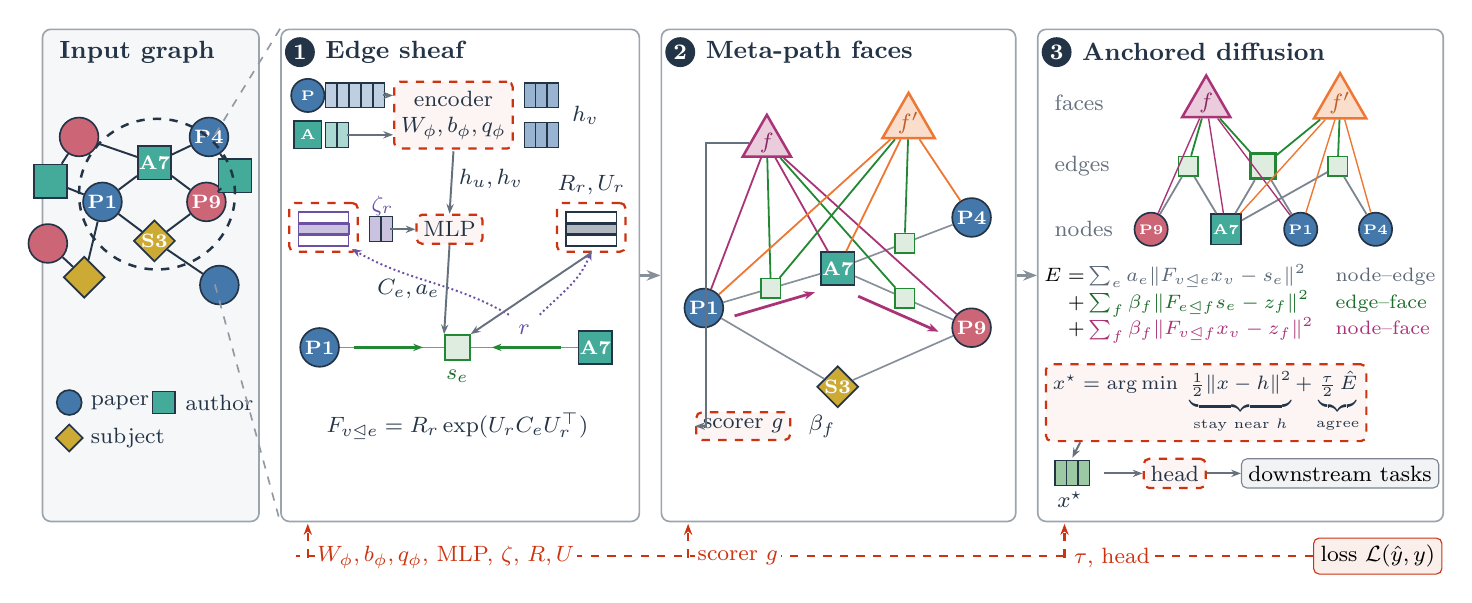
\begin{tikzpicture}
\def\WI{2.75}\def\WA{4.55}\def\WB{4.5}\def\WC{5.15}\def\G{0.28}\def\H{6.25}
\pgfmathsetmacro{\xA}{\WI+\G}\pgfmathsetmacro{\xB}{\xA+\WA+\G}\pgfmathsetmacro{\xC}{\xB+\WB+\G}
\node[stage,minimum width=\WI cm,minimum height=\H cm,fill=ink!4] (BI) at (0,0) {};
\node[sname] at (0.1,-0.3) {Input graph};
\node[stage,minimum width=\WA cm,minimum height=\H cm] (B1) at (\xA,0) {};
\node[stage,minimum width=\WB cm,minimum height=\H cm] (B2) at (\xB,0) {};
\node[stage,minimum width=\WC cm,minimum height=\H cm] (B3) at (\xC,0) {};
\foreach \i/\t in {1/Edge sheaf,2/Meta-path faces,3/Anchored diffusion}{
  \node[stnum] at ($(B\i.north west)+(0.25,-0.3)$) {\i};
  \node[sname] at ($(B\i.north west)+(0.45,-0.3)$) {\t};}
% ================= input
\begin{scope}[shift={(-0.02,-0.75)},scale=0.66]
 \node[pS,fill=cA] (iP1) at (1.2,-2.2) {P1};
 \node[aS] (iA7) at (2.2,-1.45) {A7};
 \node[sS] (iS3) at (2.2,-2.95) {S3};
 \node[pS,fill=cB] (iP9) at (3.2,-2.2) {P9};
 \node[pS,fill=cA] (iP4) at (3.25,-0.95) {P4};
 \node[pS,fill=cB] (iP2) at (0.75,-0.95) {};
 \node[aS] (iA2) at (0.2,-1.8) {};
 \node[pS,fill=cA] (iP6) at (3.45,-3.8) {};
 \node[sS] (iS4) at (0.85,-3.65) {};
 \node[pS,fill=cB] (iP7) at (0.15,-3.0) {};
 \node[aS] (iA5) at (3.75,-1.7) {};
 \draw[ed] (iP1)--(iA7) (iA7)--(iP9) (iA7)--(iP4) (iP1)--(iS3) (iS3)--(iP9)
   (iA2)--(iP2) (iA2)--(iP1) (iS3)--(iP6) (iP2)--(iA7) (iS4)--(iP7) (iS4)--(iP1) (iA5)--(iP9) (iA5)--(iP4);
 \draw[ink,dashed,line width=.9pt] (2.25,-2.05) ellipse (1.5 and 1.45);
\end{scope}
\node[pS,fill=cA,minimum size=9pt] at (0.35,-4.75) {}; \node[lab,anchor=west] at (0.5,-4.75) {paper};
\node[aS,minimum size=8pt] at (1.55,-4.75) {}; \node[lab,anchor=west] at (1.7,-4.75) {author};
\node[sS,minimum size=10pt] at (0.35,-5.2) {}; \node[lab,anchor=west] at (0.5,-5.2) {subject};
\draw[dashed,ink!50,line width=.6pt] (2.2,-1.35)--(B1.north west);
\draw[dashed,ink!50,line width=.6pt] (2.2,-3.25)--(B1.south west);
% ================= 1 edge sheaf
\begin{scope}[shift={(\xA,0)}]
 \node[pS,fill=cA,minimum size=12pt,font=\tiny\bfseries] (eP) at (0.35,-0.85) {P};
 \node[aS,minimum size=10pt,font=\tiny\bfseries] (eA) at (0.35,-1.35) {A};
 \bars{eP}{0.15,0}{5}{cA!35} \bars{eA}{0.15,0}{2}{cAu!45}
 \node[learn,minimum width=1.25cm,minimum height=0.85cm] (enc) at (2.2,-1.1) {encoder\\$W_{\phi},b_{\phi},q_{\phi}$};
 \draw[arr] (1.3,-0.85)--(enc.west|-0,-0.85); \draw[arr] (0.85,-1.35)--(enc.west|-0,-1.35);
 \bars{enc.east}{0.05,0.25}{3}{cA!55} \bars{enc.east}{0.05,-0.25}{3}{cA!55}
 \node[lab,anchor=west] at ($(enc.east)+(0.62,0)$) {$h_v$};
 % edge with its relation r
 \node[pS,fill=cA] (aP1) at (0.5,-4.05) {P1};
 \node[aS] (aA7) at (4.0,-4.05) {A7};
 \node[est,minimum size=9pt] (se) at (2.25,-4.05) {};
 \draw[nedge] (aP1)--(se)--(aA7);
 \draw[mp] ($(aP1)!0.25!(se)$)--($(aP1)!0.75!(se)$); \draw[mp] ($(aA7)!0.25!(se)$)--($(aA7)!0.75!(se)$);
 \node[lab,text=grn!80!black,anchor=north] at (se.south) {$s_e$};
 \node[font=\footnotesize\itshape,text=rel] (rr) at (3.1,-3.82) {$r$};
 % relation embedding table and per-relation frames
 \ptable{zt}{0.55,-2.55}{rel}{}
 \node[learn,fill=none,fit={($(zt)+(-0.4,0.3)$)($(zt)+(0.4,-0.25)$)},inner sep=1pt] (ztbox) {};
 \bars{zt}{0.5,0.0}{2}{rel!35}
 \node[lab,text=rel] at ($(zt)+(0.75,0.3)$) {$\zeta_r$};
 \ptable{rt}{3.95,-2.55}{ink}{}
 \node[learn,fill=none,fit={($(rt)+(-0.4,0.3)$)($(rt)+(0.4,-0.25)$)},inner sep=1pt] (rtbox) {};
 \node[lab,anchor=south] at ($(rt)+(0,0.32)$) {$R_r,U_r$};
 \draw[look] (rr.north west) to[out=150,in=-30] ($(zt)+(0.36,-0.25)$);
 \draw[look] (rr.north east) to[out=45,in=-110] ($(rt)+(0,-0.27)$);
 \node[learn] (mlp) at (2.15,-2.55) {MLP};
 \draw[arr] ($(zt)+(0.85,0)$)--(mlp.west);
 \draw[arr] ($(enc.south)+(0,-0.02)$)--node[lab,right=-1pt,pos=.45]{$h_u,h_v$}(mlp.north);
 \draw[arr] (mlp.south)--node[lab,left=-1pt,pos=.5]{$C_e,a_e$}(se.north west);
 \draw[arr] (rtbox.south)--(se.north east);
 \node[lab] at (2.25,-5.05) {$F_{v\trianglelefteq e}=R_r\exp(U_rC_eU_r^{\top})$};
\end{scope}
% ================= 2 meta-path faces
\begin{scope}[shift={(\xB,0)}]
 \node[pS,fill=cA] (bP1) at (0.55,-3.55) {P1};
 \node[aS] (bA7) at (2.25,-3.05) {A7};
 \node[pS,fill=cB] (bP9) at (3.95,-3.8) {P9};
 \node[pS,fill=cA] (bP4) at (3.95,-2.4) {P4};
 \node[sS] (bS3) at (2.25,-4.55) {S3};
 \draw[nedge] (bP1)--(bA7) (bA7)--(bP9) (bA7)--(bP4) (bP1)--(bS3) (bS3)--(bP9);
 \node[est] (q1) at ($(bP1)!0.5!(bA7)$) {}; \node[est] (q2) at ($(bA7)!0.5!(bP9)$) {}; \node[est] (q3) at ($(bA7)!0.5!(bP4)$) {};
 \draw[walk=fcF] ($(bP1)!0.2!(bA7)+(0.05,-0.2)$)--($(bP1)!0.8!(bA7)+(0.05,-0.2)$);
 \draw[walk=fcF] ($(bA7)!0.2!(bP9)+(-0.08,-0.2)$)--($(bA7)!0.8!(bP9)+(-0.08,-0.2)$);
 \node[face=fcF] (F1) at (1.35,-1.45) {$f$};
 \node[face=fcG] (F2) at (3.15,-1.2) {$f'$};
 \foreach \n in {bP1,bA7,bP9} \draw[cpl=fcF] (F1)--(\n);
 \foreach \e in {q1,q2} \draw[cpl=grn] (F1)--(\e);
 \foreach \n in {bP1,bA7,bP4} \draw[cpl=fcG] (F2)--(\n);
 \foreach \e in {q1,q3} \draw[cpl=grn] (F2)--(\e);
 \node[learn] (gsc) at (1.05,-5.05) {scorer $g$};
 \draw[arr] (F1.west) -- ++(-0.55,0) |- (gsc.west);
 \node[lab,anchor=west] (bf) at ($(gsc.east)+(0.1,0)$) {$\beta_f$};
\end{scope}
% ================= 3 anchored diffusion
\begin{scope}[shift={(\xC,0)}]
 \node[lab,anchor=west,text=ink!70] at (0.1,-0.95) {faces};
 \node[lab,anchor=west,text=ink!70] at (0.1,-1.75) {edges};
 \node[lab,anchor=west,text=ink!70] at (0.1,-2.55) {nodes};
 \node[face=fcF,minimum size=16pt] (zf) at (2.15,-0.95) {$f$};
 \node[face=fcG,minimum size=16pt] (zg) at (3.85,-0.95) {$f'$};
 \node[pS,fill=cB,minimum size=12pt,font=\tiny\bfseries] (n9) at (1.45,-2.55) {P9};
 \node[aS,minimum size=11pt,font=\tiny\bfseries] (n7) at (2.4,-2.55) {A7};
 \node[pS,fill=cA,minimum size=12pt,font=\tiny\bfseries] (n1) at (3.35,-2.55) {P1};
 \node[pS,fill=cA,minimum size=12pt,font=\tiny\bfseries] (n4) at (4.3,-2.55) {P4};
 \node[est] (e97) at (1.92,-1.75) {}; \node[est,minimum size=9pt,line width=1pt] (e71) at (2.87,-1.75) {}; \node[est] (e74) at (3.82,-1.75) {};
 \draw[cpl=ink!60] (n9)--(e97) (n7)--(e97) (n7)--(e71) (n1)--(e71) (n7)--(e74) (n4)--(e74);
 \draw[cpl=grn] (zf)--(e97) (zf)--(e71) (zg)--(e71) (zg)--(e74);
 \foreach \n in {n9,n7,n1} \draw[cpl=fcF,line width=.5pt] (zf)--(\n);
 \foreach \n in {n1,n7,n4} \draw[cpl=fcG,line width=.5pt] (zg)--(\n);
 % energy, term by term
 \node[font=\scriptsize,anchor=north west,inner sep=1pt] (eq1) at (0.05,-2.95) {$\begin{array}{@{}r@{\,}l@{\quad}l@{}}
 E= & \textcolor{ink!75}{\sum_e a_e\|F_{v\trianglelefteq e}x_v-s_e\|^2} & \textcolor{ink!75}{\text{node--edge}}\\[1pt]
 + & \textcolor{grn!80!black}{\sum_f\beta_f\|F_{e\trianglelefteq f}s_e-z_f\|^2} & \textcolor{grn!80!black}{\text{edge--face}}\\[1pt]
 + & \textcolor{fcF}{\sum_f\beta_f\|F_{v\trianglelefteq f}x_v-z_f\|^2} & \textcolor{fcF}{\text{node--face}}
 \end{array}$};
 \node[learn,font=\scriptsize,anchor=north west] (sol) at (0.1,-4.25) {$x^\star=\arg\min\ \underbrace{\tfrac12\|x-h\|^2}_{\text{stay near }h}+\underbrace{\tfrac{\tau}{2}\,\hat E}_{\text{agree}}$};
 \bars{0.15,-5.65}{0,0}{3}{grn!45}
 \node[lab] at (0.42,-5.98) {$x^\star$};
 \draw[arr] ($(sol.south west)+(0.45,0)$)--(0.45,-5.45);
 \node[learn] (head) at (1.75,-5.65) {head};
 \draw[arr] (0.85,-5.65)--(head.west);
 \node[draw=ink!60,rounded corners=2pt,fill=ink!6,font=\footnotesize,inner sep=2.5pt] (ds) at (3.85,-5.65) {downstream tasks};
 \draw[arr] (head.east)--(ds.west);
\end{scope}
\draw[flow] (B1.east)--(B2.west); \draw[flow] (B2.east)--(B3.west);
% ================= loss and what it updates
\pgfmathsetmacro{\yL}{-\H-0.45}
\node[draw=lrn,fill=lrn!8,rounded corners=2pt,font=\footnotesize,inner sep=2.5pt,anchor=east] (loss) at (\xC+\WC,\yL) {loss $\mathcal{L}(\hat y,y)$};
\draw[lrn,dashed,line width=.8pt] (loss.west)--(\xA+0.2,\yL);
\foreach \b/\dx/\t in {B1/0.35/{$W_\phi,b_\phi,q_\phi$, MLP, $\zeta$, $R,U$},B2/0.35/{scorer $g$},B3/0.35/{$\tau$, head}}{
  \draw[-{Stealth[length=4pt]},lrn,dashed,line width=.8pt] ($(\b.south west)+(\dx,-0.45)$)--($(\b.south west)+(\dx,-0.02)$);
  \node[font=\footnotesize,text=lrn,anchor=west,fill=white,inner sep=1pt] at ($(\b.south west)+(\dx+0.08,-0.45)$) {\t};}
\end{tikzpicture}
\end{document}
